% !TEX root = main.tex

\section{Learning Framework}
\label{sec:learning_framework}

Designing a physics-informed attention mechanism requires balancing expressive non-local capacity with optimization stability. The C-PINN learning framework builds upon a custom un-normalized Cross-Attention module connected to a symmetric global latent basis. Architectural and training hyperparameters were systematically selected via hyperparameter tuning using Optuna's Tree-structured Parzen Estimator (TPE) paired with Median Pruning. Key Optuna-tuned components are indicated by a blue star marker ($\nasmarker$).

\begin{figure*}[t]
    \centering
    \begin{subfigure}{\textwidth}
        \centering
        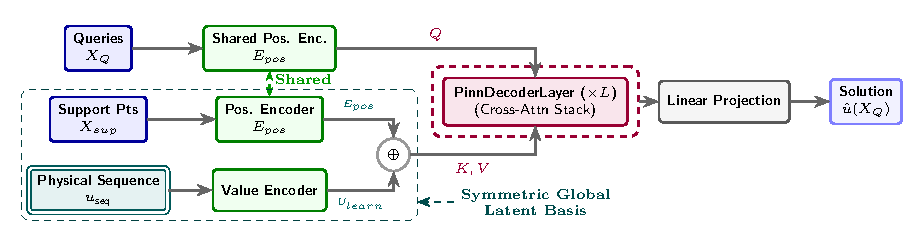
\includegraphics[width=0.92\textwidth]{figures/tlp_architecture.pdf}
        \caption{Overall macro-architecture of CrossPINN (C-PINN), depicting the baseline MLP stream interlinked with the Cross-Attention memory corrector.}
        \label{fig:c_pinn_macro_arch}
    \end{subfigure}
    \vspace{0.3cm}
    \begin{subfigure}{\textwidth}
        \centering
        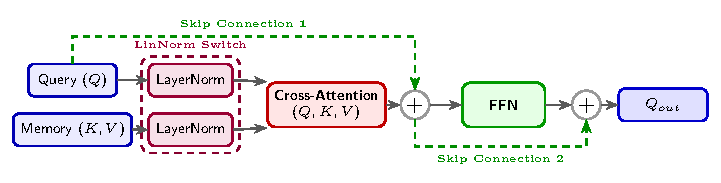
\includegraphics[width=0.92\textwidth]{figures/modules_architecture.pdf}
        \caption{Detailed micro-architecture of the custom \texttt{PinnDecoderLayer}, highlighting the optional LinNorm query/key normalization switch and un-normalized residual skip connections.}
        \label{fig:pinn_decoder_layer_micro}
    \end{subfigure}
    \caption{Complete schematic representation of the C-PINN framework: (a) Macro-scale hybrid architecture; (b) Micro-scale \texttt{PinnDecoderLayer} building block.}
    \label{fig:c_pinn_full_architecture}
\end{figure*}

\subsection{Symmetric Global Latent Basis}
To model historical memory in Volterra operators, spatial queries attend to a globally accessible latent memory matrix. Rather than decoupling spatial coordinates from latent states, C-PINN constructs a symmetric joint spatial-latent basis~\cite{jaegle2021perceiverio}:
\begin{equation}
    \text{Memory} = E_{pos}(X_{sup})\nasmarker + U_{learn} \in \mathbb{R}^{N_{sup} \times H},
    \label{eq:latent_basis}
\end{equation}
where $E_{pos}(X_{sup})$ provides deterministic positional embeddings for spatial support anchors $X_{sup}$, and $U_{learn} \in \mathbb{R}^{N_{sup} \times H}$ is a latent value matrix representing the solution basis over the support anchors. Summing spatial and value representations ensures content-aware attention: queries $X_Q$ attend to historical states based on both physical proximity and latent solution characteristics.

\subsection{Latent Solution Parameterization and Dynamic Warm-Start}
To force a physical interpretation of $U_{learn} \in \mathbb{R}^{N_{sup} \times H}$ as a latent solution basis over the domain, we structure the matrix using a spatial solution sequence $u_{\text{seq}}(X_{sup}) = \text{MLP}(X_{sup}) \in \mathbb{R}^{N_{sup} \times 1}$ evaluated by a pre-trained baseline MLP at the support anchors, projected via a linear value encoder $\text{ValEnc}(\cdot)$:
\begin{equation}
    U_{learn} = \text{ValEnc}(u_{\text{seq}}) = u_{\text{seq}} W_{val} + b_{val}.
\end{equation}

During the initial phase of training, the solution sequence $u_{\text{seq}}$ is kept frozen to the baseline MLP values for a set number of epochs ($E_{\text{unfreeze}}\nasmarker$). This allows the network to first optimize the attention mechanism and positional encodings around the baseline physical field before fine-tuning the solution representation itself.

Since we could not determine \textit{a priori} whether optimizing the 1D physical sequence or the full 2D latent matrix was superior, we let Optuna select between two unfreezing parameterization modes$\nasmarker$:
\begin{enumerate}
    \item \textbf{Sequence Parameterization:} Unfreezes the 1D physical sequence $u_{\text{seq}} \in \mathbb{R}^{N_{sup} \times 1}$, which is projected through the learnable $\text{ValEnc}(\cdot)$ layer.
    \item \textbf{Direct Latent Matrix Parameterization:} Unfreezes the full $N_{sup} \times H$ matrix $U_{learn}$ directly, granting the optimizer maximum feature capacity for high-dimensional residual refinement.
\end{enumerate}

Furthermore, because initializing $U_{learn}$ with MLP ``hints'' introduces a strong physical inductive bias that might either accelerate convergence or excessively restrict representation capacity, we left the activation of Warm-Start as an explicit Neural Architecture Search (NAS) dimension$\nasmarker$. If Warm-Start is disabled, $U_{learn}$ is initialized randomly and trained end-to-end from epoch 1.

\subsection{Positional Encoding Variants}
To map continuous spatial coordinates into high-dimensional latent space without spectral bias, C-PINN leverages a positional encoder $E_{pos}(\cdot)\nasmarker$. Rather than hardcoding a single structure, the NAS space includes five standard encoding mechanisms adopted directly from literature:
\begin{itemize}
    \item \textbf{Random Fourier Features (RFF):} Projects coordinates using a static Gaussian frequency matrix to enforce isotropic spatial distance metrics.
    \item \textbf{Learnable Fourier Features (LFF):} Dynamically optimizes spatial frequency bands via backpropagation.
    \item \textbf{MLP Encoder:} A standard two-layer feedforward network with GELU activations for generic non-linear spatial mapping.
    \item \textbf{Sinusoidal MLP (SIREN):} Employs periodic activations with a tunable scale hyperparameter $\omega_0\nasmarker$ to capture high-frequency physical gradients.
    \item \textbf{Radial Basis Functions (RBF):} Maps coordinates relative to learnable Gaussian centers and scale factors for localized spatial activations.
\end{itemize}

\subsection{Custom Cross-Attention and Decoder Stack}
Standard PyTorch Transformer layers (\texttt{nn.TransformerDecoderLayer}) enforce external LayerNormalization on hidden features and residual skip connections, while \texttt{nn.MultiheadAttention} lacks mechanisms to selectively normalize Query and Key projections. In physics-informed regression, applying LayerNorm across spatial feature dimensions forces activations to zero mean and unit variance, destroying absolute spatial scales and dampening higher-order Autograd derivatives.

To resolve these limitations, we designed a custom decoder architecture featuring two normalization controls:
\begin{enumerate}
    \item \textbf{Residual LayerNorm Removal:} External LayerNorm operations on decoder inputs and skip connections are replaced with identity mappings, preserving uncorrupted physical solution magnitudes and derivative scales.
    \item \textbf{Query/Key Normalization Switch:} To evaluate whether normalizing Query ($Q = Q W_Q$) and Key ($K = K W_K$) projections stabilizes logit dynamics, we introduced an internal query/key normalization switch as a NAS dimension$\nasmarker$.
\end{enumerate}

When query and key normalization is disabled, raw geometric inner products drive attention scoring:
\begin{equation}
    \text{Attn}(Q, K, V) = \text{Softmax}\left(\frac{(Q W_Q) (K W_K)^T}{\sqrt{d_k}}\right) V W_V.
    \label{eq:linnorm_attn}
\end{equation}
While the codebase supports lower-triangular causal attention masking ($y_j \le x$), causal masking was left unconstrained in our primary benchmark evaluations.

The complete Cross-Attention decoder comprises a stack of $L\nasmarker$ identical decoder layers ($L \in [1, 4]$ tuned via Optuna). Within each layer, intermediate feature representations pass through the Cross-Attention block followed by a Feed-Forward Network (FFN), with internal residual skip connections bypassing both blocks to guarantee stable gradient propagation through deep decoder stacks (Fig.~\ref{fig:c_pinn_full_architecture}b). Finally, the refined latent features $Q_{\text{lat}} \in \mathbb{R}^{M \times H}$ exiting the decoder stack are projected back to the physical solution space via a simple linear projection layer ($\text{Linear}: \mathbb{R}^H \to \mathbb{R}^1$).

\subsection{MLP-Residual Correction Framework}
To combine the strong inductive bias of MLPs for local differential dynamics with the non-local integration capacity of attention, C-PINN formulates the hybrid residual architecture$\nasmarker$:
\begin{equation}
    \hat{u}_\theta(x) = \text{MLP}(x) + \Delta u_{\text{Attn}}(x),
\end{equation}
where $\text{MLP}(x)$ models the macroscopic physical field and $\Delta u_{\text{Attn}}(x)$ predicts fine-grained Volterra memory corrections (Fig.~\ref{fig:c_pinn_full_architecture}a).

\subsection{Optimization Strategy and Hyperparameter Search Space}
Training is performed by minimizing a composite loss function balancing differential/integral residuals and boundary constraints:
\begin{equation}
    \mathcal{L}_{\text{total}} = \mathcal{L}_{\text{IDE}} + \lambda_{\text{BC}} \mathcal{L}_{\text{BC/IC}}.
\end{equation}
To prevent gradient dominance between loss components, constraint weight $\lambda_{\text{BC}}$ is dynamically updated using Relative Loss Balancing with Random Lookback (ReLoBRaLo)~\cite{relobralo2021}. Smooth $C^\infty$ activation functions$\nasmarker$ ($\text{activation} \in \{\text{GELU}, \text{Tanh}, \text{SiLU}\}$) are employed across all layers to ensure continuous Autograd derivatives without non-physical singularities.

Optimization is performed using the AdamW optimizer. Optimization is bounded by a maximum of $10,000$ epochs paired with an Early Stopping mechanism (patience of $500$ epochs, minimum delta threshold of $10^{-5}$).

Architectural hyperparameter optimization is conducted systematically using Optuna TPE across the search space:
\begin{itemize}
    \item \textbf{Latent Dimensions ($H$):} $H \in \{32, 64, 128\}$.
    \item \textbf{Attention Heads ($h$):} $h \in \{2, 4, 8\}$ (constrained such that $H \bmod h = 0$).
    \item \textbf{Decoder Layers ($L$):} $L \in \{1, 2, 3, 4\}$.
    \item \textbf{Support Anchors ($N_{\text{sup}}$):} $N_{\text{sup}} \in \{32, 64, 128\}$.
    \item \textbf{Learning Rate ($\text{lr}$):} Log-uniform float $\text{lr} \in [5 \times 10^{-4}, 5 \times 10^{-2}]$.
    \item \textbf{Weight Decay ($\text{wd}$):} Log-uniform float $\text{wd} \in [10^{-6}, 10^{-4}]$.
    \item \textbf{Warm-Start Unfreeze Epoch ($E_{\text{unfreeze}}$):} $E_{\text{unfreeze}} \in \{2, 1000, 2000, 3000\}$.
\end{itemize}